\chapter{Visualization Methods}
\label{Chapter2}

The purpose of our research is to visualize the subspace of the real world in which any objects could be inserted by surveillance cameras. We take up ordinary perspective cameras for surveillance cameras in this research. We propose to insert ``visual aids'' into real images captured by the mobile camera. We take up five kinds of visual aids in this paper. First we discuss the elements of visualization of viewing fields in section \ref{VisualizationRequirements}, then the detailed definitions of the visual aids are given in section \ref{VisualizationMethods}.

%------------------------------------------------------------------------------

\section{Visualization Elements}
\label{VisualizationRequirements}

Viewing volume of a projective camera is defined by an infinite half cone, one apex of which corresponds to the focal point of the camera. Because real computers cannot have unlimited resources, in practical computer 3D technology we usually limit the bottom of the cone by a far clip plane or by boundary surfaces which may cut the viewing volume, then limit the top of the cone even more by a near clip plane. This results in a frustum (figure \ref{fig:ViewingVolume}). In this research we abstract the viewing volume for visualization by the term ``viewing field''.

\begin{figure}[htbp]
	\centering
	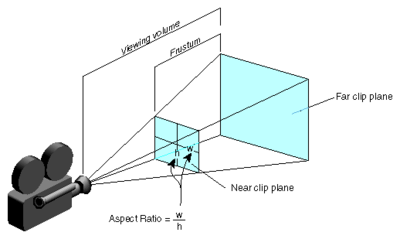
\includegraphics{./Primitives/viewing_volume.png}
	\rule{35em}{0.5pt}
	\caption[Viewing volume of camera]{Viewing volume of camera}
	\label{fig:ViewingVolume}
\end{figure}

There may be many methods for visualizing the viewing fields, not limited to the ones discussed in the next section. But for a method to find practical use in outdoor MR, it should be able to be implemented (see section \ref{UseCases} to have an illustration) so that it meets the following basic qualitative requirements, expressed in the ``it should'' tongue of most Domain Specific Languages of the Behavior Driven Development methodology in software engineering:

\begin{itemize}
	\item It should be easy to understand when users see the visualized viewing fields of surveillance cameras.
	\item It should work in realtime. When users change the position or orientation of the mobile device, the MR video displayed on the screen of the mobile device should simultaneously change accordingly to the movement of the camera with no or little delay.
	\item It should have good accuracy. In order to correctly overlay visual aids onto the original video frames taken at the user side, the position and orientation of the mobile camera must be estimated within a small registration error.
	\item It should be robust to disturbance in outdoor environment. Some of the disturbance that may arise in real situations are passers in front of the mobile camera and GPS signal noise/weakness. For example, in outdoor environment, there may be bicycle riders passing by and they may temporarily occlude the mobile camera. Another example is that if the system uses GPS device, the GPS signal strength may change a lot when users walk from an open space to a space shadowed by trees or buildings.
\end{itemize}

We must take the above requirements into account when implementing the prototype in chapter \ref{Chapter3}.

%------------------------------------------------------------------------------

\section{Visualization Methods}
\label{VisualizationMethods}

In all the five visualization methods, in order to emphasize the boundary of the viewing fields of the surveillance camera, we draw four straight lines to visualize the edges of the cone in figure \ref{fig:ViewingVolume}. The way we draw the five sides and the inside space of the cone gives us various visualization methods. A good side effect when drawing the four straight lines is that the position of the camera can be inferred because it is the only intersection point of the lines.

\subsection{Volume Method}

The most direct method to visualize the viewing field is simply visualizing the viewing volume (figure \ref{fig:VolumeMethod}) in alpha blending (see-through) fashion. However, the volume usually occupies parts of the mobile device's screen, especially if the user is inside the viewing volume, hence it may be hard to be understood.

\begin{figure}[htbp]
	\centering
	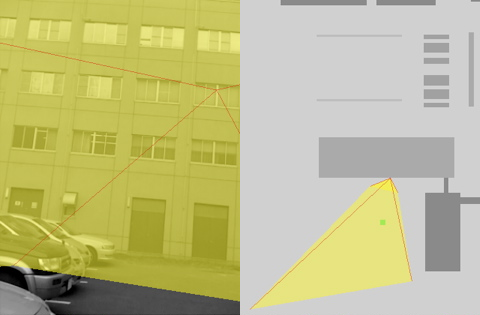
\includegraphics[width=14cm]{./Primitives/theory_volume.png}
	\rule{35em}{0.5pt}
	\caption[Volume method]{The viewing field of a surveillance camera on the building is being visualized using the volume method. The user's position is indicated by the green dot.}
	\label{fig:VolumeMethod}
\end{figure}

\subsection{Shadow Method}
\label{ShadowMethod}

The fact that the frame captured by a surveillance camera can be thought to be a perspective projection of the volume into the near plane of the frustum gives us another method, shadow method. The shadow casts the virtual shadow created by the light positioned at the focal-point of the camera and the near plane of the frustum (figure \ref{fig:ShadowMethod}). This method may give more understandable visualization.

\begin{figure}[htbp]
	\centering
	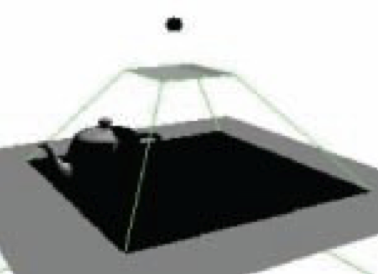
\includegraphics[width=14cm]{./Primitives/theory_shadow.png}
	\rule{35em}{0.5pt}
	\caption[Shadow method]{The viewing field of a surveillance camera on the building is being visualized using the shadow method. The user's position is indicated by the green dot.}
	\label{fig:ShadowMethod}
\end{figure}

There are various ways to render the shadow, the two popular ones are shadow mapping \cite{Reference7} \cite{Reference8} and volume shadow \cite{Reference9}.

\subsection{Contour Method}

An alternative method is to only visualize the contours of the shadow (figure \ref{fig:ContourMethod}) to reduce the occlusion of the scene by the visual aid CG object. Rendering only the contour is much lighter than rendering the whole shadow, thus this method is supposed to be much faster than the shadow method.

\begin{figure}[htbp]
	\centering
	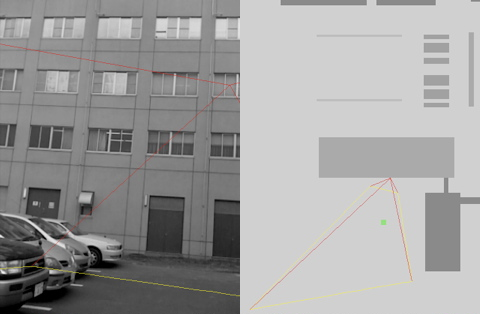
\includegraphics[width=14cm]{./Primitives/theory_contour.png}
	\rule{35em}{0.5pt}
	\caption[Contour method]{The viewing field of a surveillance camera on the building is being visualized using the contour method. The user's position is indicated by the green dot.}
	\label{fig:ContourMethod}
\end{figure}

\subsection{Arrow Method}

In some cases, a person may want to know the relative distances from points inside the shadow (section \ref{ShadowMethod}) to the camera, in addition to its viewing field itself. To visualize this information, we propose vector method that puts arrows on the shadow area as in figure \ref{fig:ArrowMethod}. In the figure, all arrows are pointing the camera, and their lengths are reverse proportional to the distance from the root of the arrows to the camera.

\begin{figure}[htbp]
	\centering
	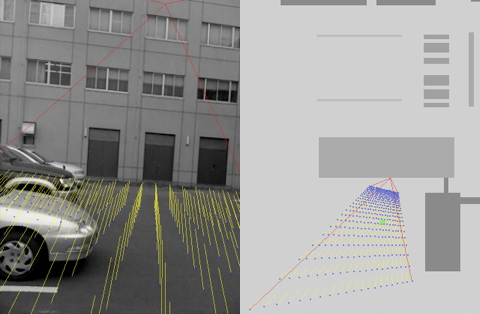
\includegraphics[width=14cm]{./Primitives/theory_arrow.png}
	\rule{35em}{0.5pt}
	\caption[Arrow method]{The viewing field of a surveillance camera on a building is being visualized using the arrow method. The arrows' roots are indicated by blue dots, the arrows' heads are not drawn for clarity. The user's position is indicated by the green dot.}
	\label{fig:ArrowMethod}
\end{figure}

\subsection{Animation Method}

This method uses a moving mesh (figure \ref{fig:AnimationMethod}) coming from the surveillance camera to the clipped end of the viewing field (or in the reverse direction) to visualize the viewing fields. This method has  many advantages:

\begin{itemize}
	\item The moving mesh starts from the surveillance camera position (or moves towards the camera). As a result the user can easily know the camera position.
	\item Even when the mobile device is fixed at a certain position and pose, the visualization effect is still helpful to understand the viewing field because of its animation.
	\item The moving mesh does not occlude the scene. As a result the user can easily see both the scene and the visualized viewing field at the same time.
\end{itemize}

\begin{figure}[htbp]
	\centering
	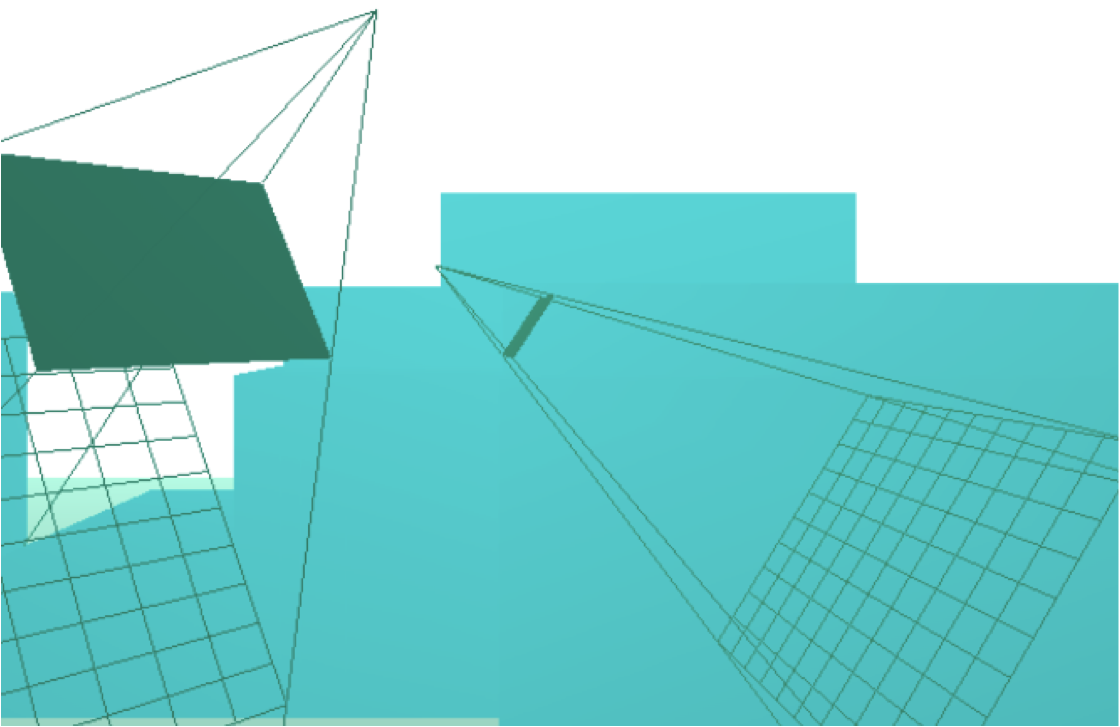
\includegraphics[width=14cm]{./Primitives/theory_animation.png}
	\rule{35em}{0.5pt}
	\caption[Animation method]{The viewing field of a surveillance camera on the building is being visualized using the animation method. The mesh is moving from the camera down to the ground. The user's position is indicated by the green dot.}
	\label{fig:AnimationMethod}
\end{figure}

To make the visual aids look more ``real'', the moving mesh stops when it touch the surface of the building walls or the ground. In order to do this, we need the model of the scene as described in the next section.

%------------------------------------------------------------------------------
\section{Scene Model}
\label{SceneModel}

In order to define the viewing field for the visualization methods in section \ref{VisualizationMethods}, we need the model of the scene. The model contains the 3D structure of the buildings (figure \ref{fig:SceneModel}) and the positions and orientations of the surveillance cameras. The model is rather simple and only contains flat planes. We do not need to have complexed ones, such as those that contain texture, because we only need a coarse-grained approximation of the viewing field. Moreover, because surveillance cameras are usually stationary, their positions and orientations are usually static.

\begin{figure}[htbp]
	\centering
	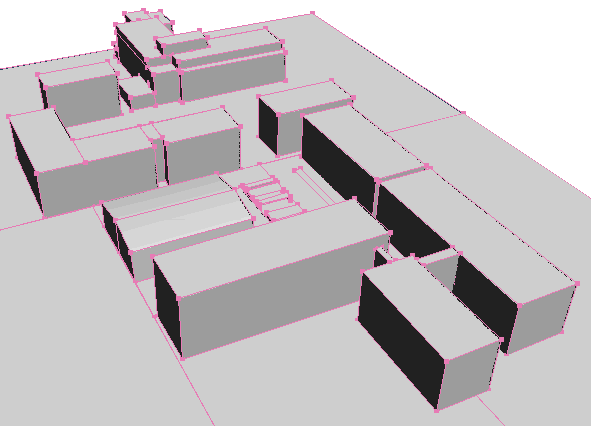
\includegraphics[width=14cm]{./Primitives/scene_model.png}
	\rule{35em}{0.5pt}
	\caption[Scene model]{3D structure of the buildings in the scene model}
	\label{fig:SceneModel}
\end{figure}

Using the scene model, we can also render visual aids in various modes as described in the next section.

%------------------------------------------------------------------------------

\section{Viewing Modes}
\label{ViewingModes}

In general it is easier to understand a thing when it is put in a context. In our case, in real scene when users see our visual aids that visualize the viewing fields of the cameras, they also see the big picture of the area around them. Consequently, if we let the users see the map of the area where they are standing, the map will help them understand the visualized viewing fields of the surrounding surveillance cameras better.

Because we have the 3D scene model as described in the previous section, we propose three viewing modes:

\begin{itemize}
	\item Real mode: In this mode frames taken by the mobile camera are overlaid with any of the visual aids.
	\item Map mode: Map of the area around the current position is displayed to let users overview the scene.
	\item First-person shooter (FPS) mode: Users can navigate the 3D world as in FPS games. Using this mode, users can virtually walk to other positions of the area to see other viewing fields of surveillance cameras there. In this mode only the scene model is rendered, video frames taken by the mobile camera are not used.
\end{itemize}

In section \ref{VisualizationMethods}, figures on the left and on the right show the screen in real mode and map mode respectively.

In order to navigate the scene in map and FPS mode, we can use the keypads on the mobile devices. However, keypads on mobile devices are usually hard to use, especially when only one hand is used to both hold the device and press the keys. When a mobile device does not have a touch screen, but it is equipped with an accelerometer (most cell phones today have one built-in) or gyrocompass, these auxiliary devices can be used for navigating around. This usage has been proved by existing applications of some game gadgets and iPhone that have those sensors. For example, in map mode the three degree-of-freedom parameters of the gyrocompass can be used as in table \ref{tb:GyrocompassNavigation}.

\begin{table}[tb]
	\begin{center}
		\caption{Using gyrocompass for navigation}
		\label{tb:GyrocompassNavigation}
		\begin{tabular}{|c|l|l|}
			\hline
			Degree-of-freedom parameter & Usage                     \\
			\hline
			Yaw                         & 360$^\circ$ rotation      \\
			Pitch                       & Forward-backward movement \\
			Roll                        & In/out zooming            \\
			\hline
		\end{tabular}
	\end{center}
\end{table}

\begin{figure}[htbp]
	\centering
	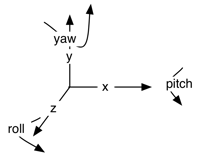
\includegraphics{./Primitives/yaw_pitch_roll.png}
	\rule{35em}{0.5pt}
	\caption[The three degree-of-freedom parameters of a gyrocompass]{The three degree-of-freedom parameters of a gyrocompass}
	\label{fig:YawPitchRoll}
\end{figure}

For devices that have multi-touch screen like the iPhone, the touch screen can be used to move, rotate, zoom in and out the map in the map viewing mode very easily.
